\subsection{Electroweak Interactions}
\label{sec:Intro_Electroweak}



% The style needs to be improved. Some places contain very chopped language.
% Consider this passage, way too “chopped”:
% > Elementary processes with W and Z bosons are shown in Fig. 3. An electric charge must be
% > conserved at any vertex. Therefore, if a charged lepton enters and radiates a W boson, a
% > neutrino or antineutrino escapes (top left in Fig. 3). That is how a W boson interacts with a
% > charged lepton and a neutrino. A lepton flavor number is always conserved in this interaction (Tab. 1).
%Consider using math mode for single character particle names, such as $c$ or $d$, to make them distinct in the text.

All electrically charged particles participate in electromagnetic interactions. Photon, the mediator of the electromagnetic interactions, is a spin-one electrically neutral massless particle. All electromagnetic interactions can be reduced to one elementary process (Fig. \ref{fig:feynmEM}, left). This process reads: an electron enters, radiates or absorbs a photon, and escapes. Although there is an electron is drawn in this figure, it can be any other charged particle as well. Such elementary process itself is forbidden by the energy conservation law but this element is a base of actual process (for example, Fig. \ref{fig:feynmEM}, middle and right). Such graphical representations of the particle physics processes are called Feynman diagrams.\\ 

\begin{figure}[htb]
  \begin{center}
    {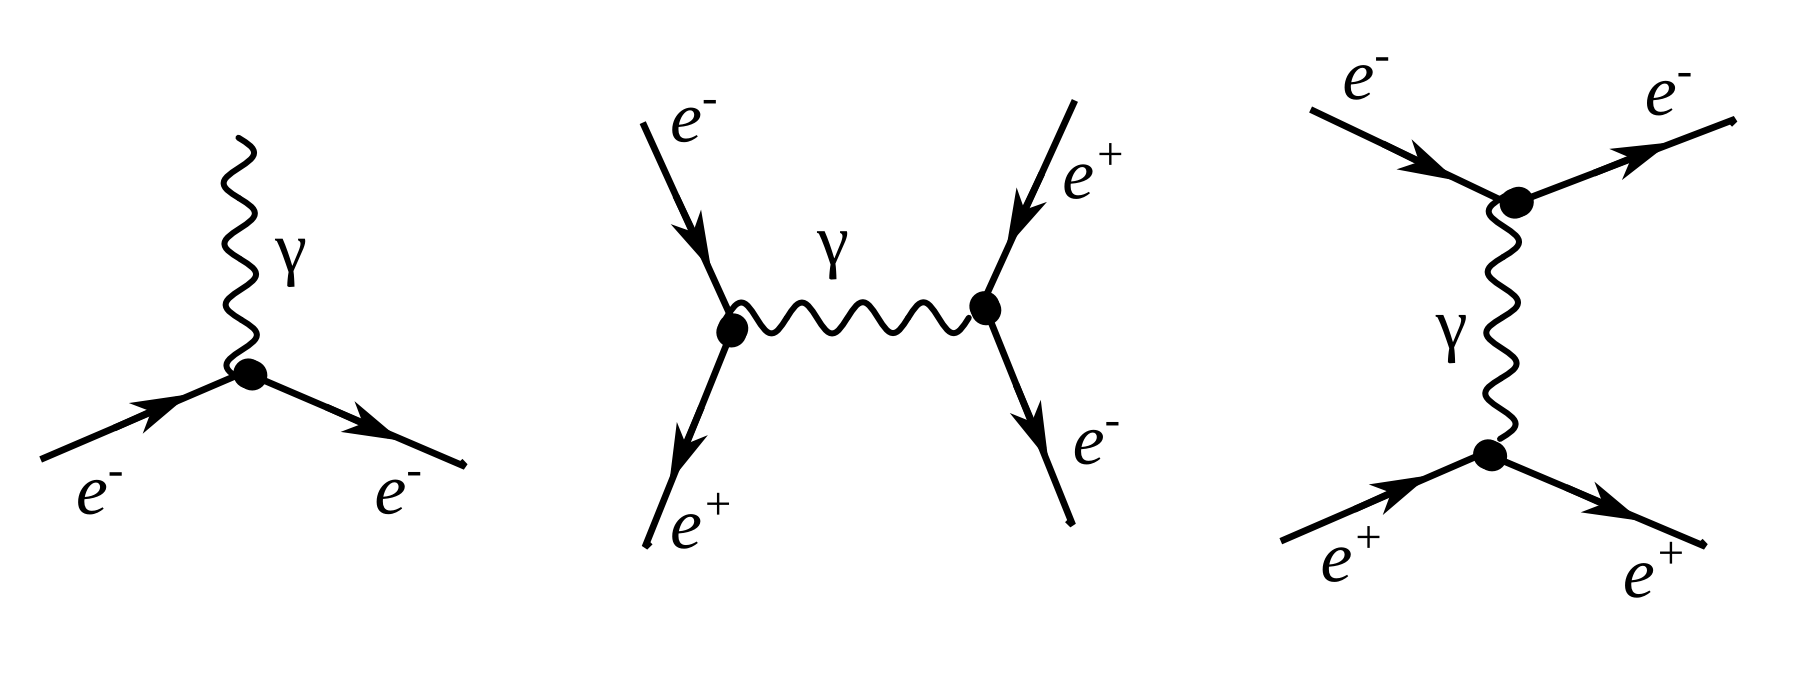
\includegraphics[width=0.90\textwidth]{../figs/Intro/feynmEM.png}}
    \caption{Electromagnetic interations}
    \label{fig:feynmEM}
  \end{center}
\end{figure}

\begin{figure}[htb]
  \begin{center}
    {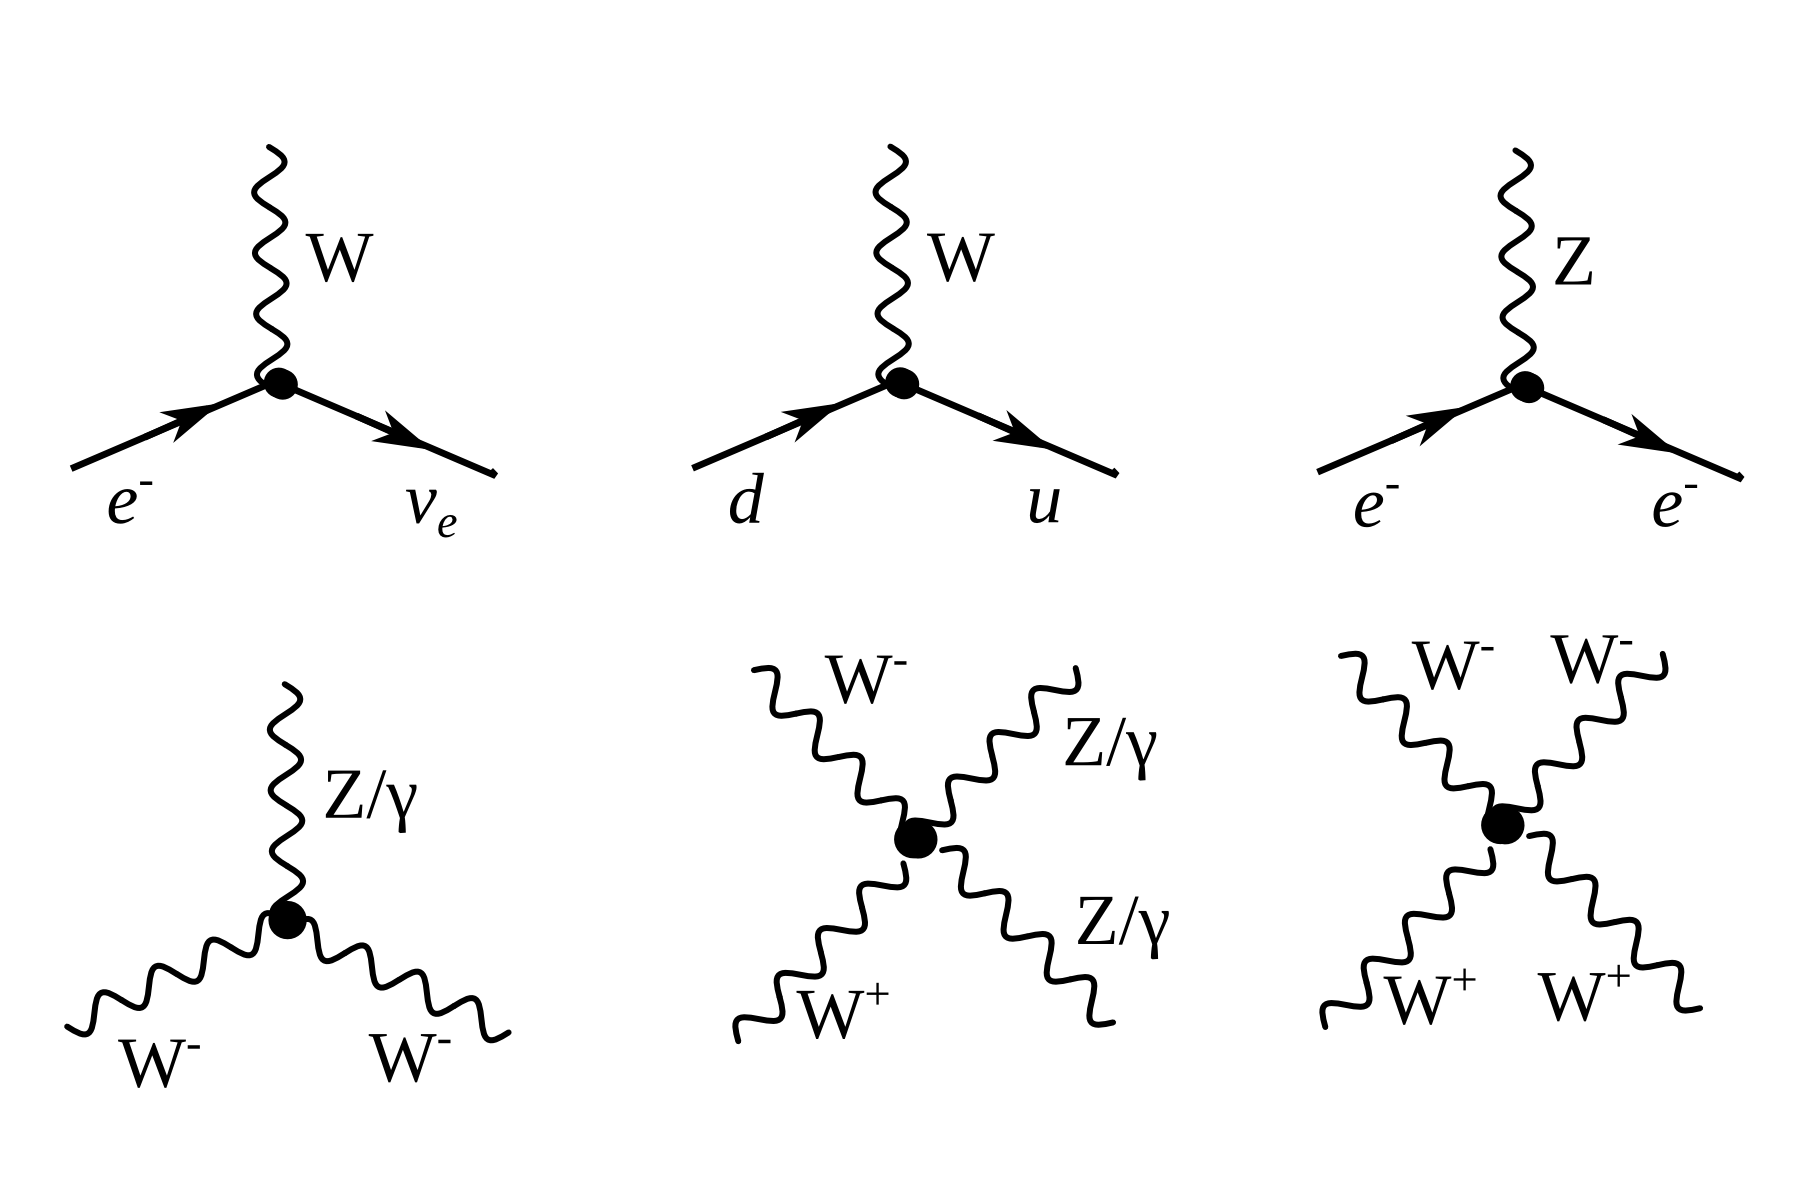
\includegraphics[width=0.90\textwidth]{../figs/Intro/feynmW.png}}
    \caption{Weak interations}
    \label{fig:feynmW}
  \end{center}
\end{figure}


As for the weak interactions, there are two kinds of them: neutral (mediated by a Z boson) and charged (mediated by a W$\pm$ boson). Elementary processes with W and Z bosons are shown in Fig. \ref{fig:feynmW}. Because the electric charge must be conserved at any vertex, a particle radiating or absorbing a W boson converts to a different particle. Thus, a charged lepton converts to a neutrino (or vice versa) as shown in Fig. \ref{fig:feynmW}, top left. A lepton flavor number is always conserved in such interactions (lepton flavor numbers assigned to different lepton are summarized in Tab. \ref{tab:LeptonFlavorNumber}), thus an electron always converts to an electron neutrino, a muon always converts to a muon neutrino etc.\\

 \begin{table}[h]
  \begin{center}
  \caption{ Lepton Flavor Number}
  \begin{tabular}{|c|c|c|c|}
     particles & $L_e$ & $L_{\mu}$ & $L_{\tau}$ \\ \hline
     $e^-,\nu_e$ &  +1  &  0  &  0  \\ \hline 
     $e^+, \bar{\nu_e}$ &  -1  &  0  &  0  \\ \hline 
     $\mu^-,\nu_{\mu}$ &  0  &  +1  &  0  \\ \hline 
     $\mu^+, \bar{\nu_{\mu}}$ &  0  &  -1  &  0  \\ \hline 
     $\tau^-,\nu_{\tau}$ &  0  &  0  &  +1  \\ \hline 
     $\tau^+, \bar{\nu_{\tau}}$ &  0  &  0  &  -1  \\ \hline 
  \end{tabular}
  \label{tab:LeptonFlavorNumber}
  \end{center}
 \end{table}

From top middle diagram in Fig. \ref{fig:feynmW} we see that if a quark with Q=-1/3 enters, then a quark with Q=+2/3 escapes and, therefore, the flavor of the quark has changed. The charged weak interaction is the only interaction which changes a quark flavor. The probability of each of three quarks with Q=+2/3 to be born is determined by the Cabibbo–Kobayashi–Maskawa matrix and is the highest for the quark of the same generation as an initial state quark (in this particular case, $d$ is the initial state quark and $u$ has the highest probability to be produced after an interaction with a W boson but $c$ and $t$ can also be produced if there is enough energy).\\

An elementary process of a neutral weak interactions is an emission of a Z boson off a fermion line (right top diagram in Fig. \ref{fig:feynmW}). An electron is shown here as an example however it also could be any lepton, antilepton, quark or antiquark. Diagrams with a Z boson are very similar to ones with a photon except a photon can only be radiated off a charged particle but a Z boson can also be radiated off a neutrino or antineutrino.\\

The bottom diagrams in Fig. \ref{fig:feynmW} are gauge coupling diagrams. Gauge couplings include self-coupling of a W boson, its interaction with Z boson and its electromagnetic radiation of a photon. WWZ, WW$\gamma$, WWZZ, WWZ$\gamma$, WW$\gamma\gamma$ and WWWW vertices are all possible in the SM.\\

Electromagnetic and weak interactions are unified by the electroweak theory. This theory considers these two forces as different manifestations of the electroweak force. While both forces can be described by very similar formalism, there is also a big difference between them: weak interactions are mediated by heavy bosons ($M_W=80$ GeV, $M_Z=91$ GeV) while electromagnetic interactions are described by a massless photon. \\

To explain this phenomenon, the Higgs mechanism was introduced. The mechanism predicted an existence of an additional boson - the Higgs boson. The Higgs boson was a missing piece of the SM for many years and was finally discovered in 2012 at the LHC by ATLAS and CMS collaborations through the processes shown in Fig.\ref{fig:higgsProduction}.\\ 

\begin{figure}[htb]
  \begin{center}
    {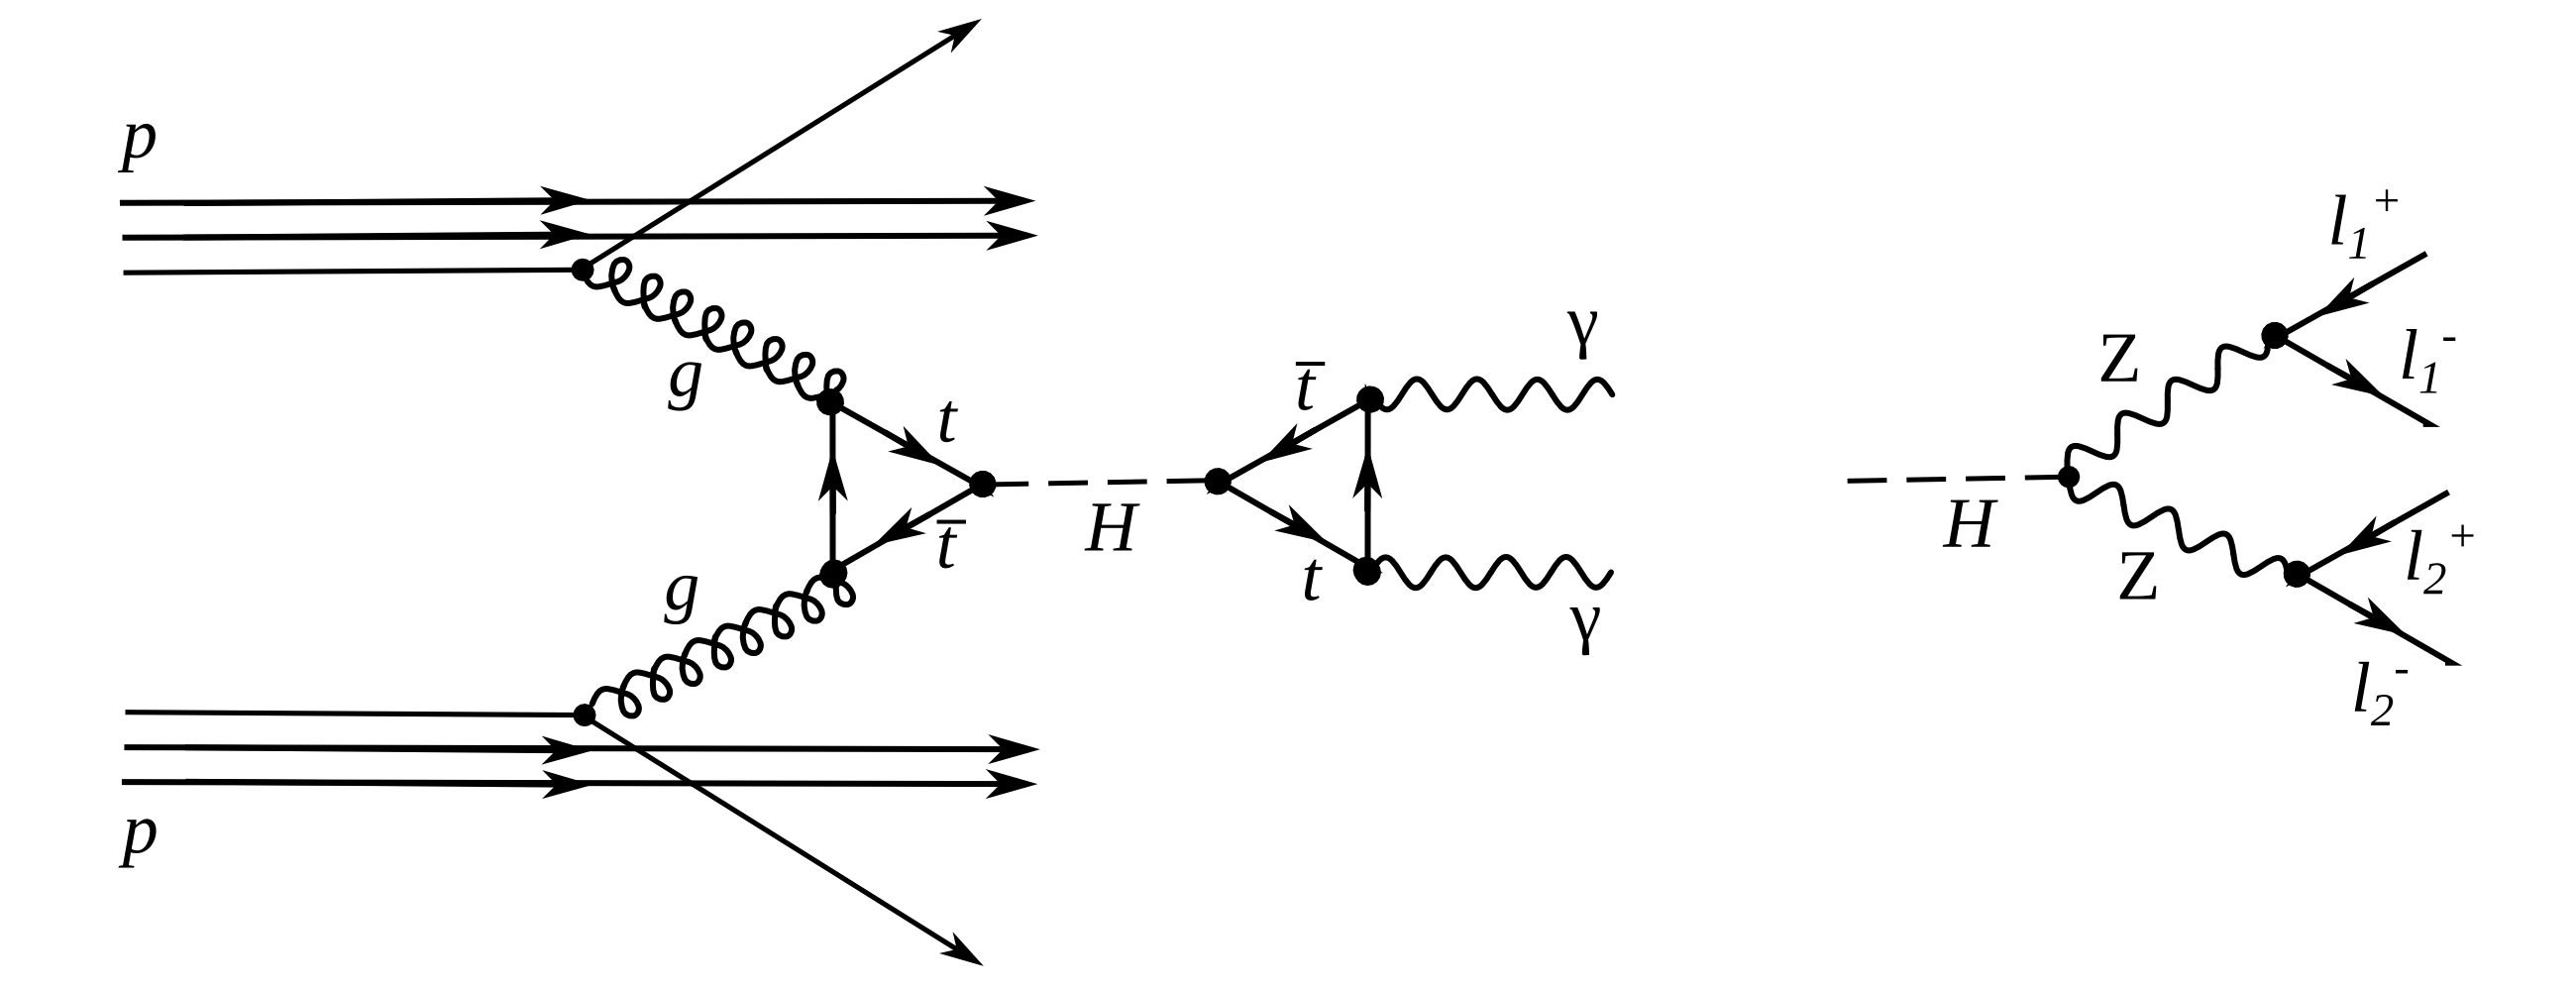
\includegraphics[width=0.95\textwidth]{../figs/Intro/FeynmanHiggs.png}}
    \caption{Higgs production and decay}
    \label{fig:higgsProduction}
  \end{center}
\end{figure}

The measurement in this dissertation is an electroweak measurement because the process involves a W boson. It includes an interaction of a W boson with leptons and quarks as well as the gauge coupling WW$\gamma$. Thus, the measurement is a good test of the SM electroweak theory.\\ 



